\chapter{Modules} \label{chap:modules}
% Structure of base module description
% - definovat nezavislost 
% - define config files (JSON, structure)
% - define communication by WebSocket and MQTT (topics)

% Structure of each module:
% - description
% - commands and responses
% - communicating with who
% - next used technology (fritzing, mongoDB, etc.)

Modules are well-encapsulated code written to provide functional and control elements (moves) above home to the user. Each module inherits from VoicehomeModule class that provide communicating interface to each module by WebSocket, MQTT and mediate writing and reading from MongoDB. Each module defines its topic for MQTT and a passport for WebSocket that subscribe from these services. Messages containing these topics or passports are passed through the engine to the modules.

Thus each module has to be created by the following approach:

\begin{enumerate}[label=\arabic*)]
    \item Create a new folder in \texttt{"voicehome\textbackslash modules\textbackslash "}, the name of this folder is the module's name.
    \item Create two mandatory files
    \begin{enumerate}
        \item \texttt{"voicehome\textbackslash modules\textbackslash <module\_name>\textbackslash metadata.json"} that include object with following variables.
        \begin{itemize}
            \item \texttt{"module\_id"}: contain the name of the module
            \item \texttt{"description"}: contain a string with a brief description of the module
            \item \texttt{"mqtt\_topics"}: contain a list of MQTT topics module wants to subscribe
            \item \texttt{"websocket\_passports"}: contain a list of WebSocket passports passing messages to the module
            \item \texttt{"moves"}: list of objects that define moves this module is capable of
            \begin{itemize}
                \item \texttt{"move\_id"}: a unique ID that follows the convention \texttt{<module\_name>\_<order\_in\_this\_list>}
                \item \texttt{"method\_name"}: contain the name of a Python function in \texttt{<module\_name>.py} called when this move is activated
                \item \texttt{"description"}: contain a brief description of the move
                \item \texttt{"calls"}: list of calls (voice commands to VoiceKit) activating this move; it is a list of lists of words (must fit the chosen logic algorithm)
            \end{itemize}
        \end{itemize}
        \item \texttt{"voicehome/modules/<module\_name>/<module\_name>.py"} that define class of module. This class have to inherit from VoicehomeModule and include all methods listed in the previous file \texttt{metadata.json}.
        
        \lstinputlisting[language=python,firstnumber=1,caption={Template for creating a new module},captionpos=b, label={lst:regex_python}]{code/module_class_template.py}
    \end{enumerate}
\end{enumerate}

After accomplishing these requirements, it is not necessary to restart the entire engine but can simply use the voice command \texttt{"načti moduly"} from the System module. Each particular module can be turned off or on using the web interface in the Modules tab, which is specified in more detail in \cref{section:modules}.

\section{Lights}

The system module provides the user commands to control lights by voice. The user not only turns on, off or blinks lights but can also identify the development boards by lighting a onboard LED on a specific board. The module keeps in memory a list of all lights with their current status and detailed description.

The onboard LEDs are mounted on the board from the factory on pin 2. The other lights have their specific wiring, but one LED is prepared for demonstration purposes, which by our definition is located in the living room and is wired according to the diagram in \cref{fig:led_schema}. 

\begin{figure}[H]
	\centering
	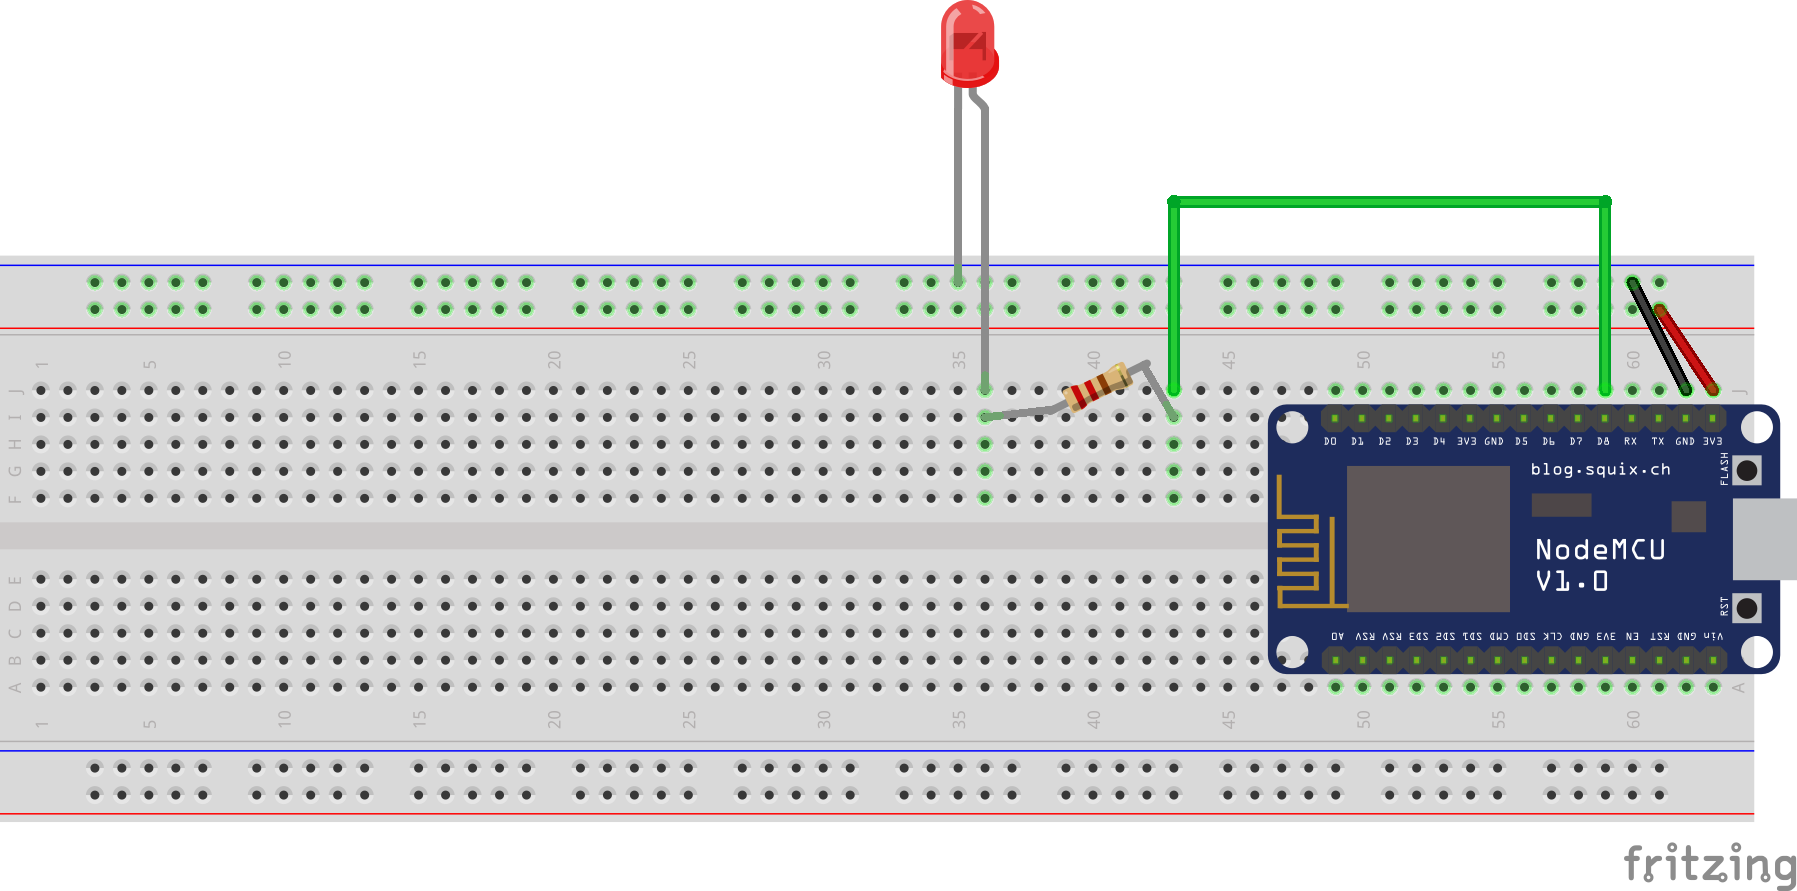
\includegraphics[width=\textwidth]{img/led_schema.png}
	\caption{LED "living room" wiring diagram}
	\label{fig:led_schema}
\end{figure}

\subsection{Voice commands}

\begin{table}[H]
	\centering
    \resizebox{\textwidth}{!}{\begin{tabular}{|l|l|l|}
        \hline
        \multicolumn{1}{c}{\bfseries ID} & \multicolumn{1}{c}{\bfseries function} & \multicolumn{1}{c}{\bfseries \# calls} \\ \hline
        \multicolumn{1}{|l|}{1}  & \multicolumn{1}{l|}{Turn on all the onboard LEDs.}     & \multicolumn{1}{l|}{2} \\ \hline
        \multicolumn{1}{|l|}{2}  & \multicolumn{1}{l|}{Turn off all the onboard LEDs.}    & \multicolumn{1}{l|}{2} \\ \hline
        \multicolumn{1}{|l|}{3}  & \multicolumn{1}{l|}{Turn on the light 1}               & \multicolumn{1}{l|}{4} \\ \hline
        \multicolumn{1}{|l|}{4}  & \multicolumn{1}{l|}{Turn off the light 1}              & \multicolumn{1}{l|}{4} \\ \hline
        \multicolumn{1}{|l|}{5}  & \multicolumn{1}{l|}{Turn on the onboard LED number 1}  & \multicolumn{1}{l|}{2} \\ \hline
        \multicolumn{1}{|l|}{6}  & \multicolumn{1}{l|}{Turn off the onboard LED number 1} & \multicolumn{1}{l|}{2} \\ \hline
        \multicolumn{1}{|l|}{7}  & \multicolumn{1}{l|}{Turn on the onboard LED number 2}  & \multicolumn{1}{l|}{2} \\ \hline
        \multicolumn{1}{|l|}{8}  & \multicolumn{1}{l|}{Turn off the onboard LED number 2} & \multicolumn{1}{l|}{2} \\ \hline
        \multicolumn{1}{|l|}{9}  & \multicolumn{1}{l|}{Turn on the onboard LED number 3}  & \multicolumn{1}{l|}{2} \\ \hline
        \multicolumn{1}{|l|}{10} & \multicolumn{1}{l|}{Turn off the onboard LED number 3} & \multicolumn{1}{l|}{2} \\ \hline
        11                       & Voicekit answer which lights are turned on             & 1                      \\ \hline
    \end{tabular}}
	\caption{Voice commands of the Lights module (for detail see \cref{section:app_lights})}
	% \label{tab:mongoDB_terminology}
\end{table}

\subsection{Messages structure}
The engine uses for maintain lights following topics and messages:

\begin{itemize}
    \item "voicehome/lights/command" - to turn the light on/off
    \begin{lstlisting}[language=json,firstnumber=1,caption={Structure of JSON message to turn on/off the light in module \textit{Lights}},captionpos=b,xleftmargin=1cm]
{
    "ID":1,
    "type":"ESP_onboard",
    "set":0
}
    \end{lstlisting}
    \item "voicehome/lights/state/command" - to ask the light for state
    \begin{lstlisting}[language=json,firstnumber=1,caption={Structure of JSON message to asking for the state of the light in module \textit{Lights}},captionpos=b,xleftmargin=1cm]
{
    "ID":1,
    "type":"ESP_onboard"
}
    \end{lstlisting}
    \item "voicehome/lights/state/receive" - to receive state of the light
    \begin{lstlisting}[language=json,firstnumber=1,caption={Structure of JSON message to receive state of the light in module \textit{Lights}},captionpos=b,xleftmargin=1cm]
{
    "type":"light",
    "state":0,
    "ID":1
}
    \end{lstlisting}
\end{itemize}

\section{Sensors}

The sensors module provides the user commands to communicate directly with sensors wired to the ESP development board or ask for statistics information such as average. The sensors connected to the module are bme280 (see \cref{fig:bme280_schema}), ds18b20 (see \cref{fig:ds18b20_schema}) and tsl2591 (see \cref{fig:tsl2591_schema}). The module uses the Python library to obtain old data from the MongoDB database to calculate statistical data.

\subsection{Voice commands}

\begin{table}[H]
    \centering
    \resizebox{\textwidth}{!}{\begin{tabular}{|l|l|l|}
        \hline
        \multicolumn{1}{c}{\bfseries ID} & \multicolumn{1}{c}{\bfseries function} & \multicolumn{1}{c}{\bfseries \# calls} \\ \hline
        \multicolumn{1}{|l|}{1}  & \multicolumn{1}{l|}{Sends a command via MQTT to measure current temperature} & \multicolumn{1}{l|}{3} \\ \hline
        \multicolumn{1}{|l|}{2}  & \multicolumn{1}{l|}{Sends a command via MQTT to measure current pressure}    & \multicolumn{1}{l|}{3} \\ \hline
        \multicolumn{1}{|l|}{3}  & \multicolumn{1}{l|}{Sends a command via MQTT to measure current humidity}    & \multicolumn{1}{l|}{3} \\ \hline
        \multicolumn{1}{|l|}{4}  & \multicolumn{1}{l|}{Sends a command via MQTT to measure current illuminance} & \multicolumn{1}{l|}{3} \\ \hline
        \multicolumn{1}{|l|}{5}  & \multicolumn{1}{l|}{Voicekit answer average temperature for the last day}    & \multicolumn{1}{l|}{2} \\ \hline
        \multicolumn{1}{|l|}{6}  & \multicolumn{1}{l|}{Voicekit answer average pressure for the last day}       & \multicolumn{1}{l|}{2} \\ \hline
        \multicolumn{1}{|l|}{7}  & \multicolumn{1}{l|}{Voicekit answer average humidity for the last day}       & \multicolumn{1}{l|}{2} \\ \hline
        \multicolumn{1}{|l|}{8}  & \multicolumn{1}{l|}{Voicekit answer average illuminance for the last day}    & \multicolumn{1}{l|}{2} \\ \hline
        \multicolumn{1}{|l|}{9}  & \multicolumn{1}{l|}{Voicekit answer average temperature for the last week}   & \multicolumn{1}{l|}{2} \\ \hline
        \multicolumn{1}{|l|}{10} & \multicolumn{1}{l|}{Voicekit answer average pressure for the last week}      & \multicolumn{1}{l|}{2} \\ \hline
        \multicolumn{1}{|l|}{11} & \multicolumn{1}{l|}{Voicekit answer average humidity for the last week}      & \multicolumn{1}{l|}{2} \\ \hline
        \multicolumn{1}{|l|}{12} & \multicolumn{1}{l|}{Voicekit answer average illuminance for the last week}   & \multicolumn{1}{l|}{2} \\ \hline
    \end{tabular}}
    \caption{Voice commands of the Sensors module (for detail see \cref{section:app_sensors})} 
\end{table} 

\subsection{Messages structure}

The engine uses for maintain sensors following topics and messages:

\begin{itemize}
    \item "voicehome/sensors/temperature" - to receiving data from temperature sensors
    \begin{lstlisting}[language=json,firstnumber=1,caption={Structure of JSON message for receiving data from temperature sensors in module \textit{Sensors}},captionpos=b,xleftmargin=1cm]
{
    "location":"room_2",
    "sensor_id":"ds18b20_1",
    "state":"ok",
    "timestamp":"2021-05-15 03:18:19",
    "quantity_units":"degree",
    "temperature_value":21.5625,
    "quantity_type":"temperature",
    "owner":"jsanda"
}
    \end{lstlisting}
    \item "voicehome/sensors/illuminance" - to receiving data from illuminance sensors
    \begin{lstlisting}[language=json,firstnumber=1,caption={Structure of JSON message for receiving data from illuminance sensors in module \textit{Sensors}},captionpos=b,xleftmargin=1cm]
{
    "location":"room_1",
    "sensor_id":"tsl2591_1",
    "state":"ok",
    "timestamp":"2021-05-15 03:19:21",
    "quantity_units":"lx",
    "quantity_type":"illuminance",
    "illuminance_value":0.0,
    "owner":"jsanda"
}
    \end{lstlisting}
    \item "voicehome/sensors/pressure" - to receiving data from illuminance sensors
    \begin{lstlisting}[language=json,firstnumber=1,caption={Structure of JSON message for receiving data from pressure sensors in module \textit{Sensors}},captionpos=b,xleftmargin=1cm]
{
    "location":"room_1",
    "sensor_id":"bme280_1",
    "state":"ok",
    "timestamp":"2021-05-15 03:19:20",
    "pressure_value":965,
    "quantity_units":"hPa",
    "quantity_type":"pressure",
    "owner":"jsanda"
}
    \end{lstlisting}
    \item "voicehome/sensors/command" - to command sensor to measure current data
    \begin{lstlisting}[language=json,firstnumber=1,caption={Structure of JSON message to command sensor to measure current data in module \textit{Sensors}},captionpos=b,xleftmargin=1cm]
{
    "command":"measure_now",
    "sensor_ID":"ds18b20_1",
    "quantity_type":"temperature",
    "who_asking":"voicekit"
}
    \end{lstlisting}
%     \item "sensorsState" - to send sensors
%     \begin{lstlisting}[language=json,firstnumber=1,caption={Structure of JSON message to command sensor to measure current data in module \textit{Sensors}},captionpos=b,xleftmargin=1cm]
% {
%     "message":"sensorsState",
%     "reply":{
%         "temperature":[
%             {
%                 "room":"room_1",
%                 "room_description":"Living room",
%                 "sensor_id":"bme280_1",
%                 "description":"The temperature in the living room",
%                 "state":"ok",
%                 "timestamp":"2021-05-15 16:13:20",
%                 "location":"room_1",
%                 "value":24.63
%             },
%             {
%                 "room":"room_2",
%                 "room_description":"Hallway",
%                 "sensor_id":"ds18b20_1",
%                 "description":"The temperature in the hallway",
%                 "state":"ok",
%                 "timestamp":"2021-05-15 16:13:20",
%                 "location":"room_2",
%                 "value":22.1875
%             }
%         ]
%     }
% }
%     \end{lstlisting}
\end{itemize}


\subsection{BME280}

% The BME280 \citep{BME280_Datasheet} module is used to measure the internal temperature and barometric pressure. In addition, our variant has a humidity sensor, which could not be put into operation, probably due to a defective piece. The measuring range of this sensor is in case of ambient temperature from -40 $^{\circ}$C to +85 $^{\circ}$C, in case of humidity from 0$\%$ to 100$\%$ and in case of barometric pressure from 300 hPa to 1100 hPa. Temperature values are measured with an accuracy of ±1 $^{\circ}$C, humidity values with an accuracy of ±3$\%$ and barometric pressure values with an accuracy of ±1 Pa. The sensor is supplied with power from a 3.3 V output on the microchip and grounded to the microchip. The SDA and SCL outputs are wired to the D6 and D5 pins of the microchip to provide I2C communication. The wiring diagram of the TSL2591 sensor is shown in \cref{fig:bme280_schema}

\begin{figure}[H]
	\centering
	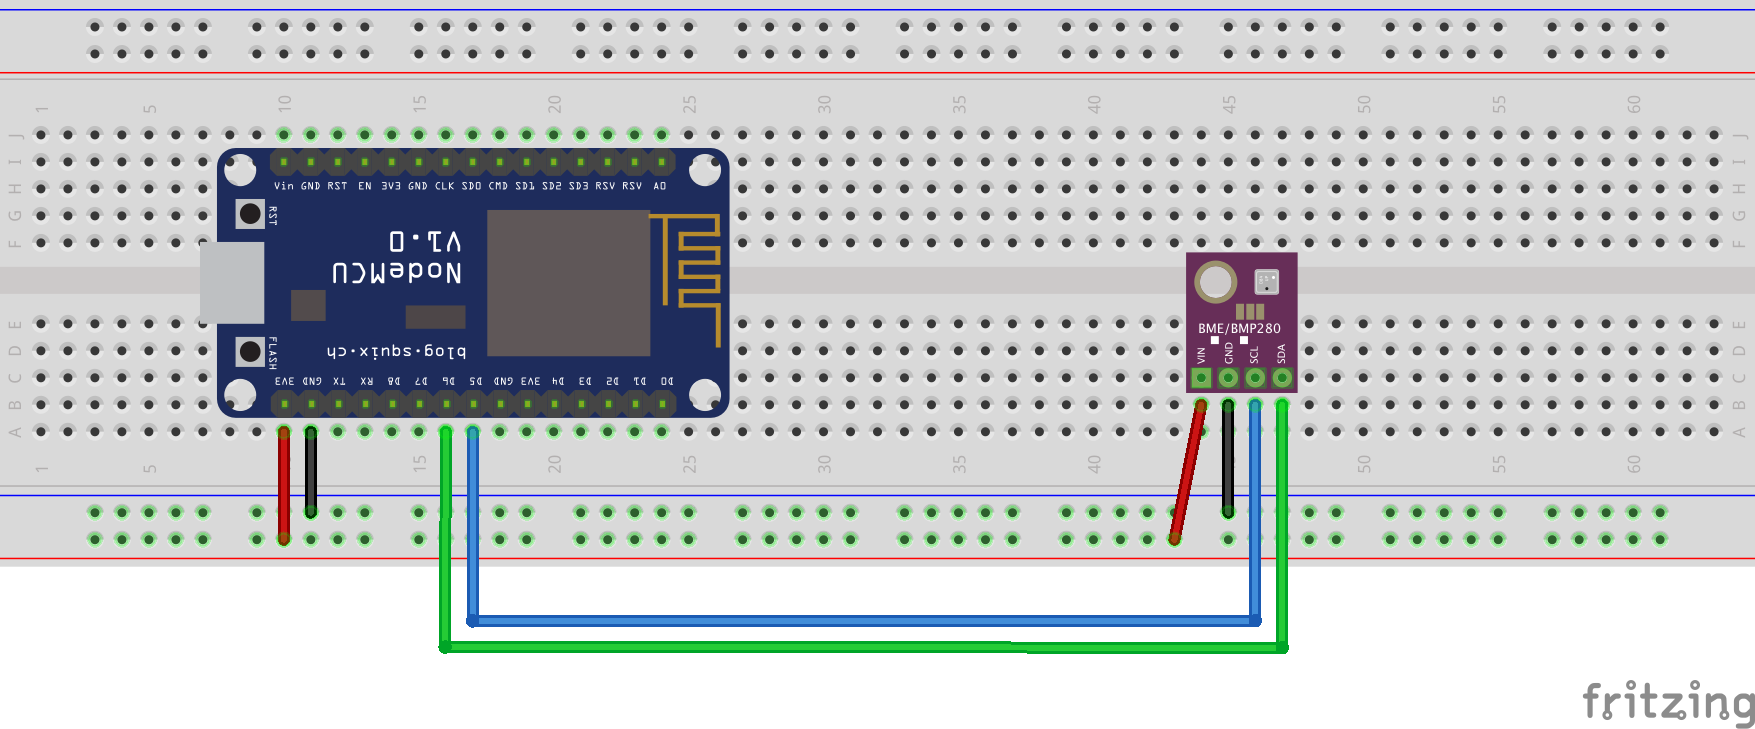
\includegraphics[width=\textwidth]{img/bme280_schema.png}
	\caption{BME 280 wiring diagram}
	\label{fig:bme280_schema}
\end{figure}


\subsection{DS18B20}

% The DS18B20 \citep{DS18B20_Datasheet} is a temperature sensor, and its waterproof variant was chosen as an illustration.  The module's output is the value of temperature in the degree Celsius unit. The sensor's measuring range is from -55 to +125 degrees with an accuracy of ± 0,5 $^{\circ}$C within limits from -10 $^{\circ}$C to +85 $^{\circ}$C. The sensor communicates via the One-Wire interface and uses one pin for data transmission. The sensor is connected to the microchip by three wires - one wire for power supply 3,3V, one for grounding and one for data communication. It is necessary to connect a resistor of resistance 4.7 k$\Omega$ to the circuit, connecting the data and power wires. The wiring diagram of the DS18B20 sensor is shown in \cref{fig:ds18b20_schema}

\begin{figure}[H]
	\centering
	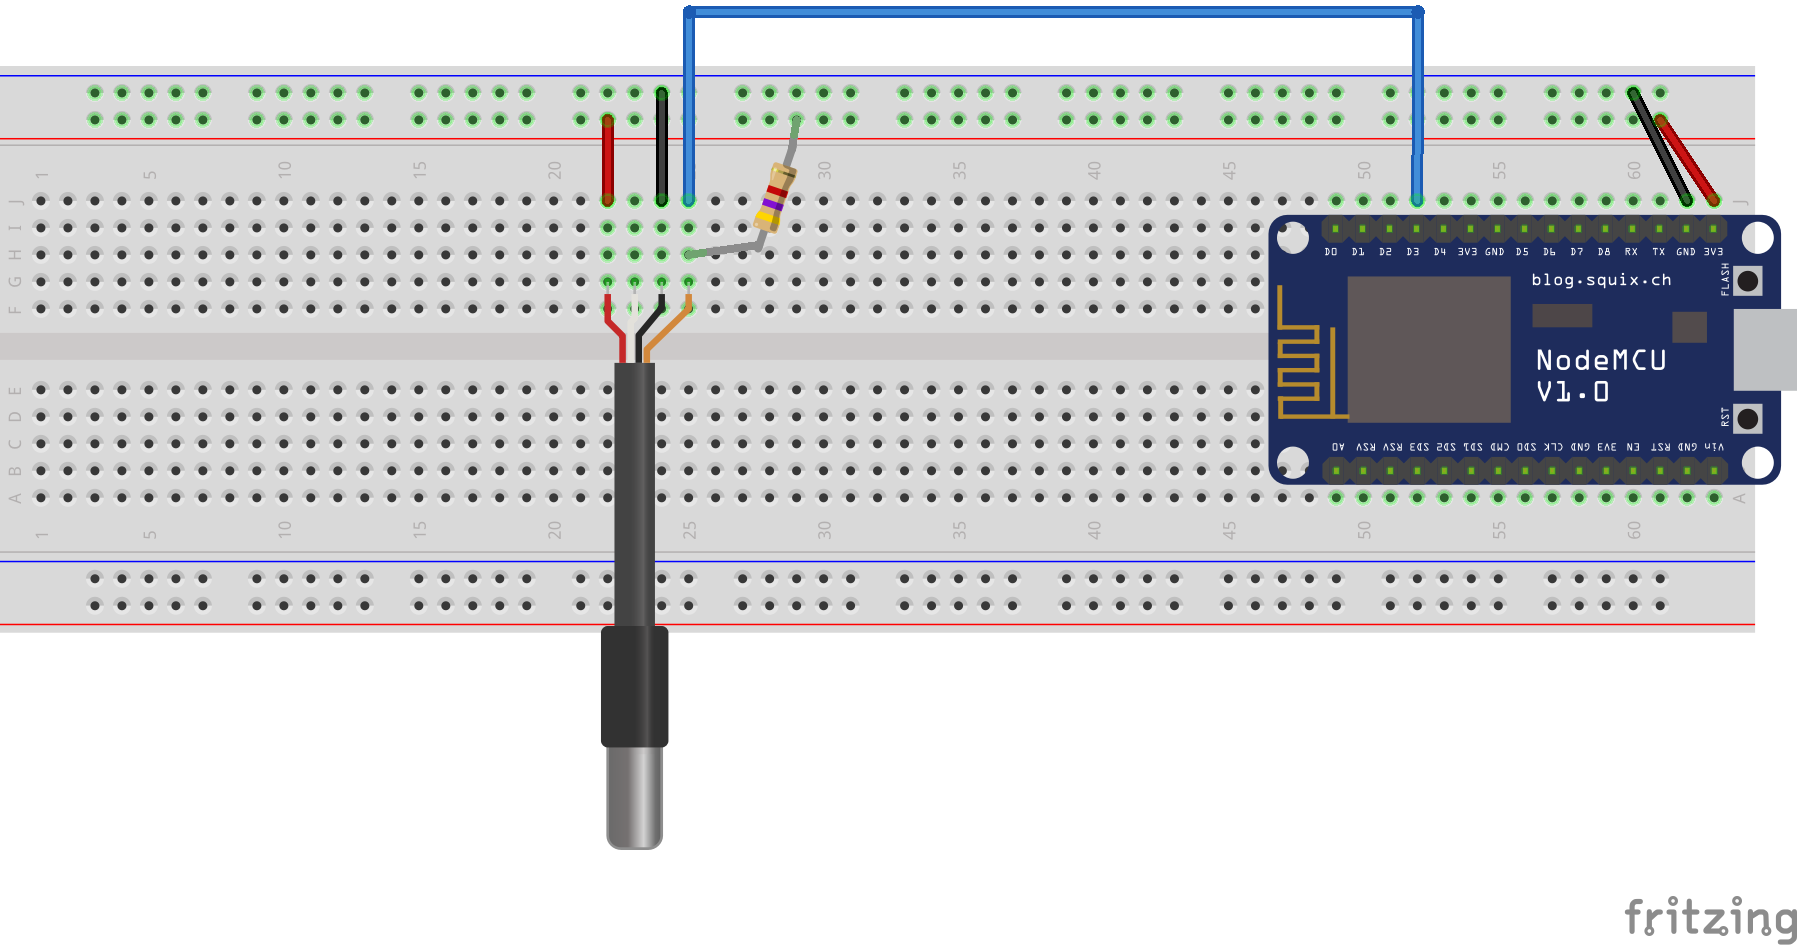
\includegraphics[width=\textwidth]{img/ds18b20_schema.png}
	\caption{DS18B20 wiring diagram}
	\label{fig:ds18b20_schema}
\end{figure}

\subsection{TSL2591}

% The TSL2591 \citep{TSL2591_Datasheet} is a light intensity sensor that converts the light intensity into a digital output transmitted by the I2C bus. The module's output is the value of light intensity in the lux unit with an accuracy of 4 decimal places, and the measuring range is from 188 $\mu$Lux to 88,000 Lux. The value of the sensor is measured to three decimal places, although it is not necessary to have such high accuracy. The module guarantees measurement accuracy in temperature conditions from -30 $^{\circ}$C to +80 $^{\circ}$C. The sensor is supplied with power from a 3.3 V output on the microchip and grounded to the microchip. The SDA and SCL outputs are wired to the D1 and D2 pins of the microchip to provide I2C communication. The wiring diagram of the TSL2591 sensor is shown in \cref{fig:tsl2591_schema}

\begin{figure}[H]
	\centering
	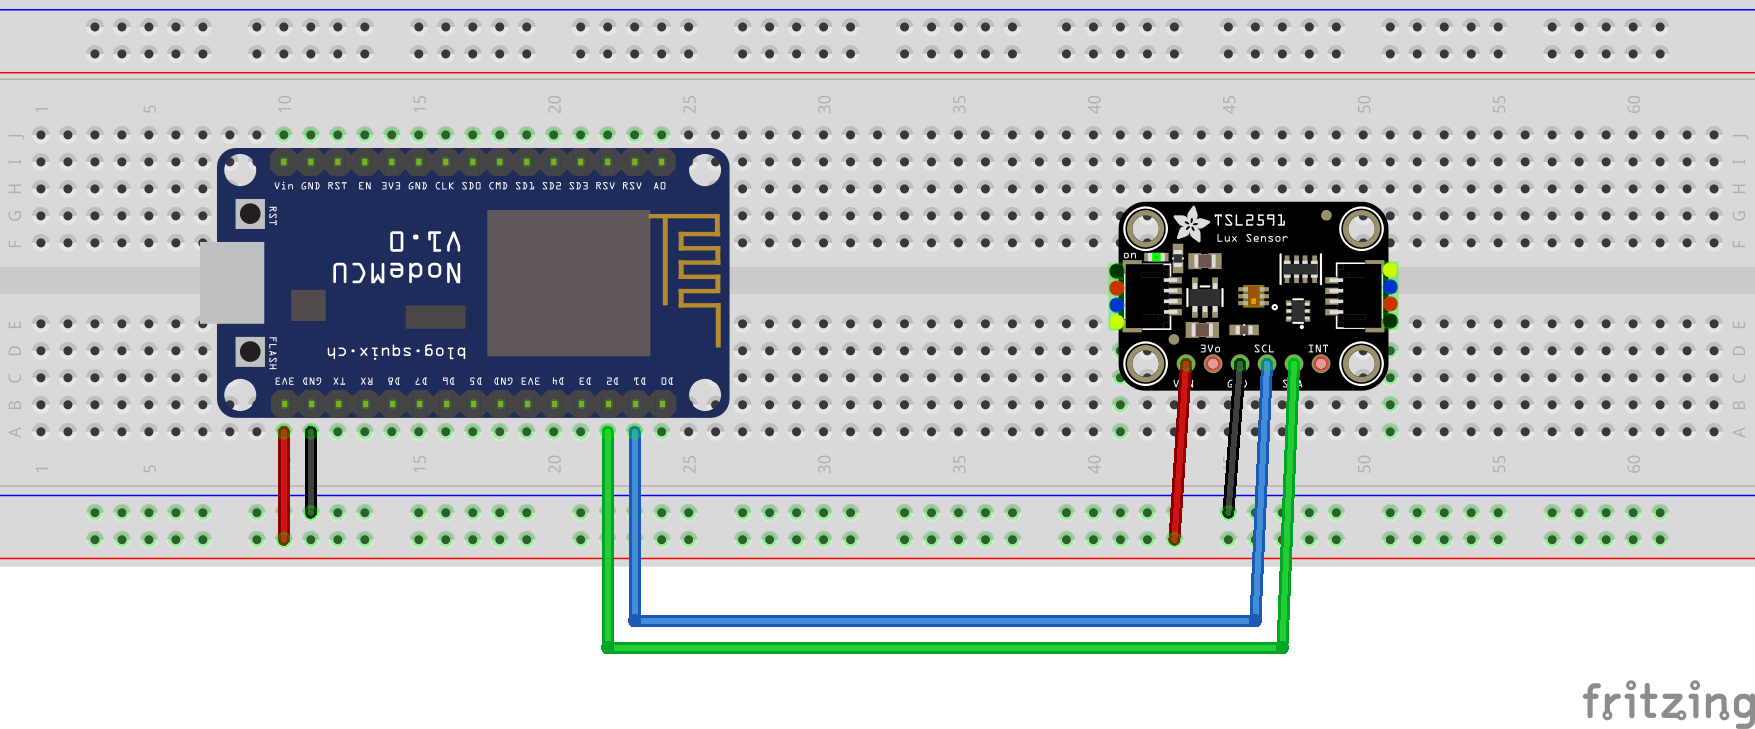
\includegraphics[width=\textwidth]{img/tsl2591_schema.png}
	\caption{TSL2591 wiring diagram}
	\label{fig:tsl2591_schema}
\end{figure}

\section{Time}

This module provides commands for manipulation with the time, such as asking for time, date, set timer. The module does not communicate with other devices. The module's functions exploit system information and information available on the Internet. To reach this information from the web is used technique call web scraping that can run the web site and suck desired pieces of information from this site. 

% A simple example of this technic is shown in \cref{lst:web_scraping_python}

% \begin{lstlisting}[language=python,firstnumber=1,caption={Simple example how to do web scraping in Python},captionpos=b, label={lst:web_scraping_python}]
%     from selenium import webdriver
%     from selenium.webdriver.chrome.options import Options

%     self.driver = webdriver.Chrome(executable_path='/usr/bin/chromedriver')
%     self.driver.get('www.seznam.cz')
% \end{lstlisting}

\subsection{Voice commands}

\begin{table}[H]
    \centering
    \resizebox{\textwidth}{!}{\begin{tabular}{|l|l|l|}
        \hline
        \multicolumn{1}{c}{\bfseries ID} & \multicolumn{1}{c}{\bfseries function} & \multicolumn{1}{c}{\bfseries \# calls} \\ \hline
        \multicolumn{1}{|l|}{1}  & \multicolumn{1}{l|}{Send command to ask the server for the current time}        & \multicolumn{1}{l|}{2}                      \\ \hline
        \multicolumn{1}{|l|}{2}  & \multicolumn{1}{l|}{Send command to ask the server for the current day of year} & \multicolumn{1}{l|}{2}                      \\ \hline
        \multicolumn{1}{|l|}{3}  & \multicolumn{1}{l|}{Send a command to the server to start timer on 3 minute}    & \multicolumn{1}{l|}{1}                      \\ \hline
        \multicolumn{1}{|l|}{4}  & \multicolumn{1}{l|}{Send a command to the server to stop timer}                 & \multicolumn{1}{l|}{2}                      \\ \hline
        \multicolumn{1}{|l|}{5}  & \multicolumn{1}{l|}{Ask the server for today's day of the week}                 & \multicolumn{1}{l|}{2}                      \\ \hline
        \multicolumn{1}{|l|}{6}  & \multicolumn{1}{l|}{Ask the server for today's sunrise time}                    & \multicolumn{1}{l|}{2}                      \\ \hline
        \multicolumn{1}{|l|}{7}  & \multicolumn{1}{l|}{Ask the server for today's sunset time}                     & \multicolumn{1}{l|}{2}                      \\ \hline
        \multicolumn{1}{|l|}{8}  & \multicolumn{1}{l|}{Ask the server for today's nameday}                         & \multicolumn{1}{l|}{2}                      \\ \hline
    \end{tabular}}
    \caption{Voice commands of the Time module (for detail see \cref{section:app_time})} 
\end{table} 

\section{System}

The system module provides the user commands to test the functionality and adjust some settings of the engine. The module communicates primarily with the engine, but it is possible to establish this communication with other devices. Like other technology, the module uses the MongoDB library from python to test the engine's database.

\subsection{Voice commands}

\begin{table}[H]
    \centering
    \resizebox{\textwidth}{!}{\begin{tabular}{|l|l|l|}
        \hline
        \multicolumn{1}{c}{\bfseries ID} & \multicolumn{1}{c}{\bfseries function} & \multicolumn{1}{c}{\bfseries \# calls} \\ \hline
        \multicolumn{1}{|l|}{1}  & \multicolumn{1}{l|}{Reloads all the modules again. A fresh refresh.}                                              & \multicolumn{1}{l|}{3}                      \\ \hline
        \multicolumn{1}{|l|}{2}  & \multicolumn{1}{l|}{Makes a testing write and read with the database.}                                            & \multicolumn{1}{l|}{3}                      \\ \hline
        \multicolumn{1}{|l|}{3}  & \multicolumn{1}{l|}{Makes a testing MQTT publish} & \multicolumn{1}{l|}{3}                      \\
        \multicolumn{1}{|l|}{}  & \multicolumn{1}{l|}{to voicehome/system/test,} &  \multicolumn{1}{l|}{}                     \\
        \multicolumn{1}{|l|}{}  & \multicolumn{1}{l|}{which this module is also subscribing} &  \multicolumn{1}{l|}{}                     \\ \hline
        \multicolumn{1}{|l|}{4}  & \multicolumn{1}{l|}{Sends a testing websocket message}                                 & \multicolumn{1}{l|}{3}                      \\
        \multicolumn{1}{|l|}{}  & \multicolumn{1}{l|}{with passport system/test.} &  \multicolumn{1}{l|}{}                     \\ \hline
    \end{tabular}}
    \caption{Voice commands of the System module (for detail see \cref{section:app_system})} 
\end{table} 

\section{Weather}

The weather module provides the user commands to answer questions about the weather. The module's functions exploit the information available on the Internet. By preprocessing the information from the Internet and replating characters like "°C" to "stupnů" or "-" to "mínus", we can then send fully synthesizable text to SpeechCloud and answer the question to the user. To reach this information from the web is used technique call web scraping that can run the web site and suck desired pieces of information from this site. Preprocessing the information uses the technique regex and essential functions such as finding text and selecting text — a simple example of how regex is used shown in \cref{lst:regex_python}.

% \lstinputlisting[language=python,firstnumber=1,caption={Simple example how to use regex in Python},captionpos=b, label={lst:regex_python}]{code/regex_example.py}

\subsection{Voice commands}

\begin{table}[H]
    \centering
    \resizebox{\textwidth}{!}{\begin{tabular}{|l|l|l|}
        \hline
        \multicolumn{1}{c}{\bfseries ID} & \multicolumn{1}{c}{\bfseries function} & \multicolumn{1}{c}{\bfseries \# calls} \\ \hline
        \multicolumn{1}{|l|}{1} & \multicolumn{1}{l|}{Getting forecast for today from www.chmi.cz.}                                           & \multicolumn{1}{l|}{2} \\ \hline
        \multicolumn{1}{|l|}{2} & \multicolumn{1}{l|}{Getting forecast for tomorrow from www.chmi.cz.}                                        & \multicolumn{1}{l|}{2} \\ \hline
        \multicolumn{1}{|l|}{3} & \multicolumn{1}{l|}{Getting forecast for monday from www.chmi.cz}   & \multicolumn{1}{l|}{2} \\ 
        \multicolumn{1}{|l|}{} & \multicolumn{1}{l|}{if it is up to four days and not today.}                                           & \multicolumn{1}{l|}{} \\ \hline
        \multicolumn{1}{|l|}{4} & \multicolumn{1}{l|}{Getting forecast for tuesday from www.chmi.cz}  & \multicolumn{1}{l|}{2} \\ 
        \multicolumn{1}{|l|}{} & \multicolumn{1}{l|}{if it is up to four days and not today.}                                           & \multicolumn{1}{l|}{} \\ \hline
        \multicolumn{1}{|l|}{5} & \multicolumn{1}{l|}{Getting forecast for wednesday from www.chmi.cz} & \multicolumn{1}{l|}{2} \\ 
        \multicolumn{1}{|l|}{} & \multicolumn{1}{l|}{if it is up to four days and not today.}                                           & \multicolumn{1}{l|}{} \\ \hline
        \multicolumn{1}{|l|}{6} & \multicolumn{1}{l|}{Getting forecast for thursday from www.chmi.cz} & \multicolumn{1}{l|}{2} \\ 
        \multicolumn{1}{|l|}{} & \multicolumn{1}{l|}{if it is up to four days and not today.}                                           & \multicolumn{1}{l|}{} \\ \hline
        \multicolumn{1}{|l|}{7} & \multicolumn{1}{l|}{Getting forecast for friday from www.chmi.cz}   & \multicolumn{1}{l|}{2} \\ 
        \multicolumn{1}{|l|}{} & \multicolumn{1}{l|}{if it is up to four days and not today.}                                           & \multicolumn{1}{l|}{} \\ \hline
        \multicolumn{1}{|l|}{8} & \multicolumn{1}{l|}{Getting forecast for saturday from www.chmi.cz} & \multicolumn{1}{l|}{2} \\ 
        \multicolumn{1}{|l|}{} & \multicolumn{1}{l|}{if it is up to four days and not today.}                                           & \multicolumn{1}{l|}{} \\ \hline
        \multicolumn{1}{|l|}{9} & \multicolumn{1}{l|}{Getting forecast for sunday from www.chmi.cz}   & \multicolumn{1}{l|}{2} \\ 
        \multicolumn{1}{|l|}{} & \multicolumn{1}{l|}{if it is up to four days and not today.}                                           & \multicolumn{1}{l|}{} \\ \hline
    \end{tabular}}
    \caption{Voice commands of the Weather module (for detail see \cref{section:app_weather})} 
\end{table} 
